\subsection{Gradient descent method}

Using the convolution notation \eqref{con010}, we consider
$$
J(v_h)=I(\nu)=\frac12\nu^TA\ast\nu-b^T\nu
$$
and 
$$
\nabla I(\nu) =A\ast \nu -b,
$$
where $A=\frac{1}{h}[-1,2, -1]$.

At the same time, let $\displaystyle u_h=\sum_{i=1}^n\mu_i\varphi_i,$
\begin{equation}\label{min}
\displaystyle u_h=\argmin_{v_h\in V_h} J(v_h)\Leftrightarrow \mu=\argmin_{\nu \in R^n} I(\nu)
\end{equation}

Noting that $\nabla I(\nu) =A\ast \nu -b$ and applying the gradient descent method to solve problem \eqref{min}, we obtain 
$$
\mu^{(m)}=\mu^{(m-1)}-\eta(A\ast \mu^{(m-1)}-b),\quad m=1,\cdots,\nu. 
$$
After $\nu$ iterations of gradient descent method, we denote the solution as $u_h^{\nu}$.

Consider the finite element discretization of Poisson equation in 1D: One very simple iterative method for \eqref{min} is the following
gradient descent method
$$
       \mu^{(m)}=\mu^{(m-1)}+\eta (b-A\ast \mu^{(m-1)}),
$$
or, for $j=1:N$, 
$$ 
\mu^{(m)}_j=\mu^{(m-1)}_j+\eta
\bigg(\beta_j-\frac{-\mu^{(m-1)}_{j-1}+2\mu^{(m-1)}_j-\mu^{(m-1)}_{j+1}}{h}\bigg),
$$
where $\eta>0$ is a positive parameter named learning rate.  

It is not so difficult to
properly choose $\eta$ so that the above iterative scheme converges,
namely for any initial guess $\mu^0$, the sequence $(\mu^{(m)})$ generated
by the above iteration converges to the exact solution $\mu$ of
\eqref{min}.

Note that
$$
        \mu=\mu+\eta (b-A\ast\mu),
$$
we get
$$
        \mu-\mu^{(m)}=(I-\eta A\ast)(\mu-\mu^{(m-1)}),
$$
or
$$
        \mu-\mu^{(m)}=(I-\eta A\ast)^m(\mu-\mu^0), m=1,2,3,\cdots
$$
As we known,
$$
(I-\eta A\ast)^m\longrightarrow 0
$$
if and only if $\rho (I-\eta A\ast)<1$. Here $\rho(B)$ is the spectral 
radius of $B$. However, $\rho (I-\eta A\ast)<1$ if and only if
$$
0< \mbox{all the eigenvalue of}~ A\ast< 2\eta^{-1}.
$$
Thus, a necessary and sufficient condition for the 
convergence is the following
$$
       0< \eta<{2\over \rho(A\ast)}.
$$
It is easy to see that
(for example, $4/h$ is an upper bound of its row sums)
$$
{4\over {h}}> \rho(A\ast).
$$
Therefore it is reasonable to make the following choice
$$
        \eta={h \over 4}
$$
and the resulting algorithm is 
\begin{equation}\Label{1dRichardson}
        \mu^{(m)}=\mu^{(m-1)}+{h\over4} (b-A\ast\mu^{(m-1)}).
\end{equation}
In the rest of this section, unless otherwise noted, we shall choose
$\eta$ as above for simplicity.

On Figure~\ref{fig:richardson} the convergence history plot of the
above gradient descent iterative method for typical application is shown.
As we see, this iterative scheme converges very slowly.

\begin{figure}[!htb]
\begin{center}
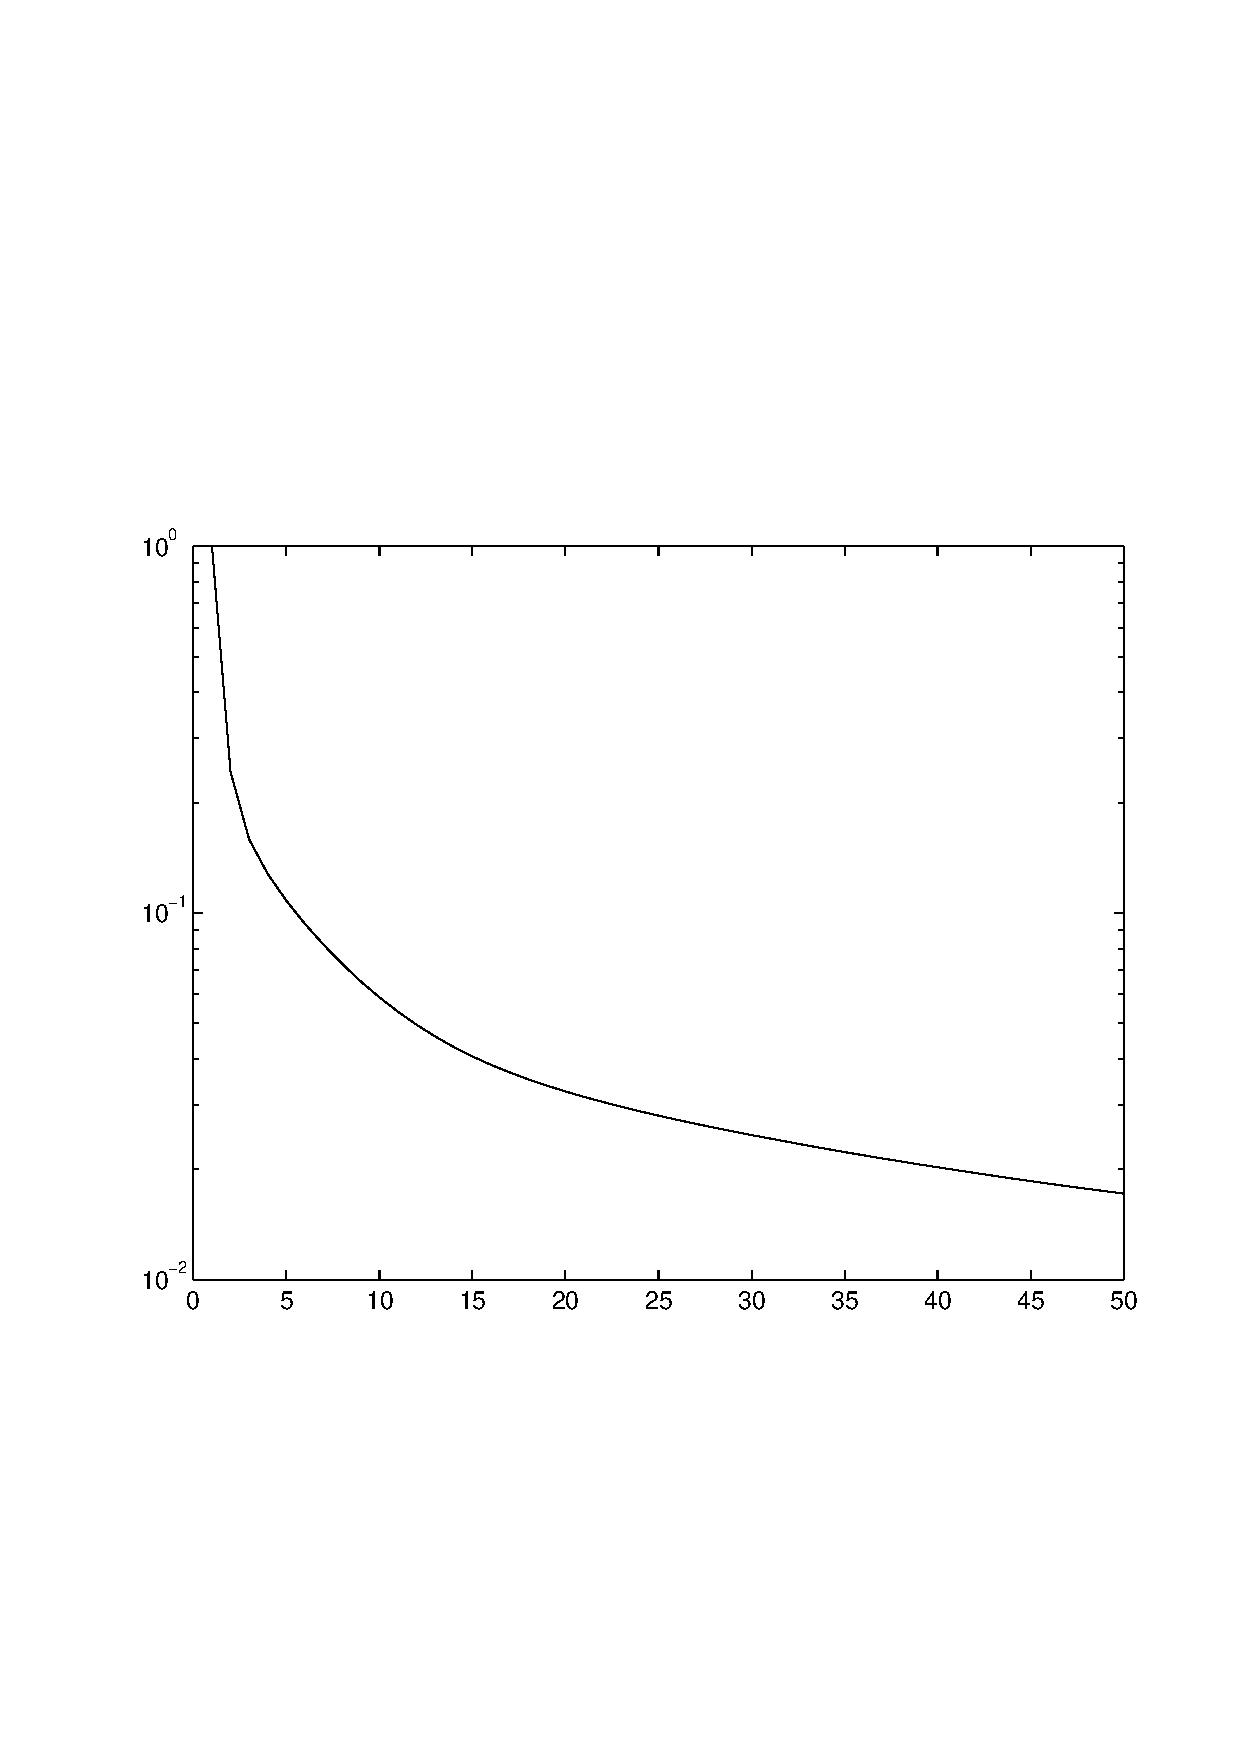
\includegraphics[height=5cm,width=3in]{pictures/richardson.pdf}
\end{center}
\caption{A picture on the GD method convergence history
\label{fig:richardson}}
\end{figure}

Our main goal is to find a way to speed up such kind of rather slowly
convergent iterative scheme.  To do that, we need to study its
convergent property in more microscopic level.  First of all, let us
now take a careful look at the convergence history picture and make
the following observation:
\begin{quote}
\underbar{\it Observation 1.}  The scheme converges rather fast in the
very beginning but then slows down after a few steps. Overall, the method 
converges very slowly. 
\end{quote}
To further understand this phenomenon, let us plot the detailed
pictures of the error functions in the first few iterations.
After a careful look at these pictures, we have the following 
observation:
\begin{quote}
\underbar{\it Observation 2.} The scheme not only converges fast in the
first few steps, but also smooth out the error function very quickly.
\end{quote}

\begin{figure}[!htb]
\begin{center}
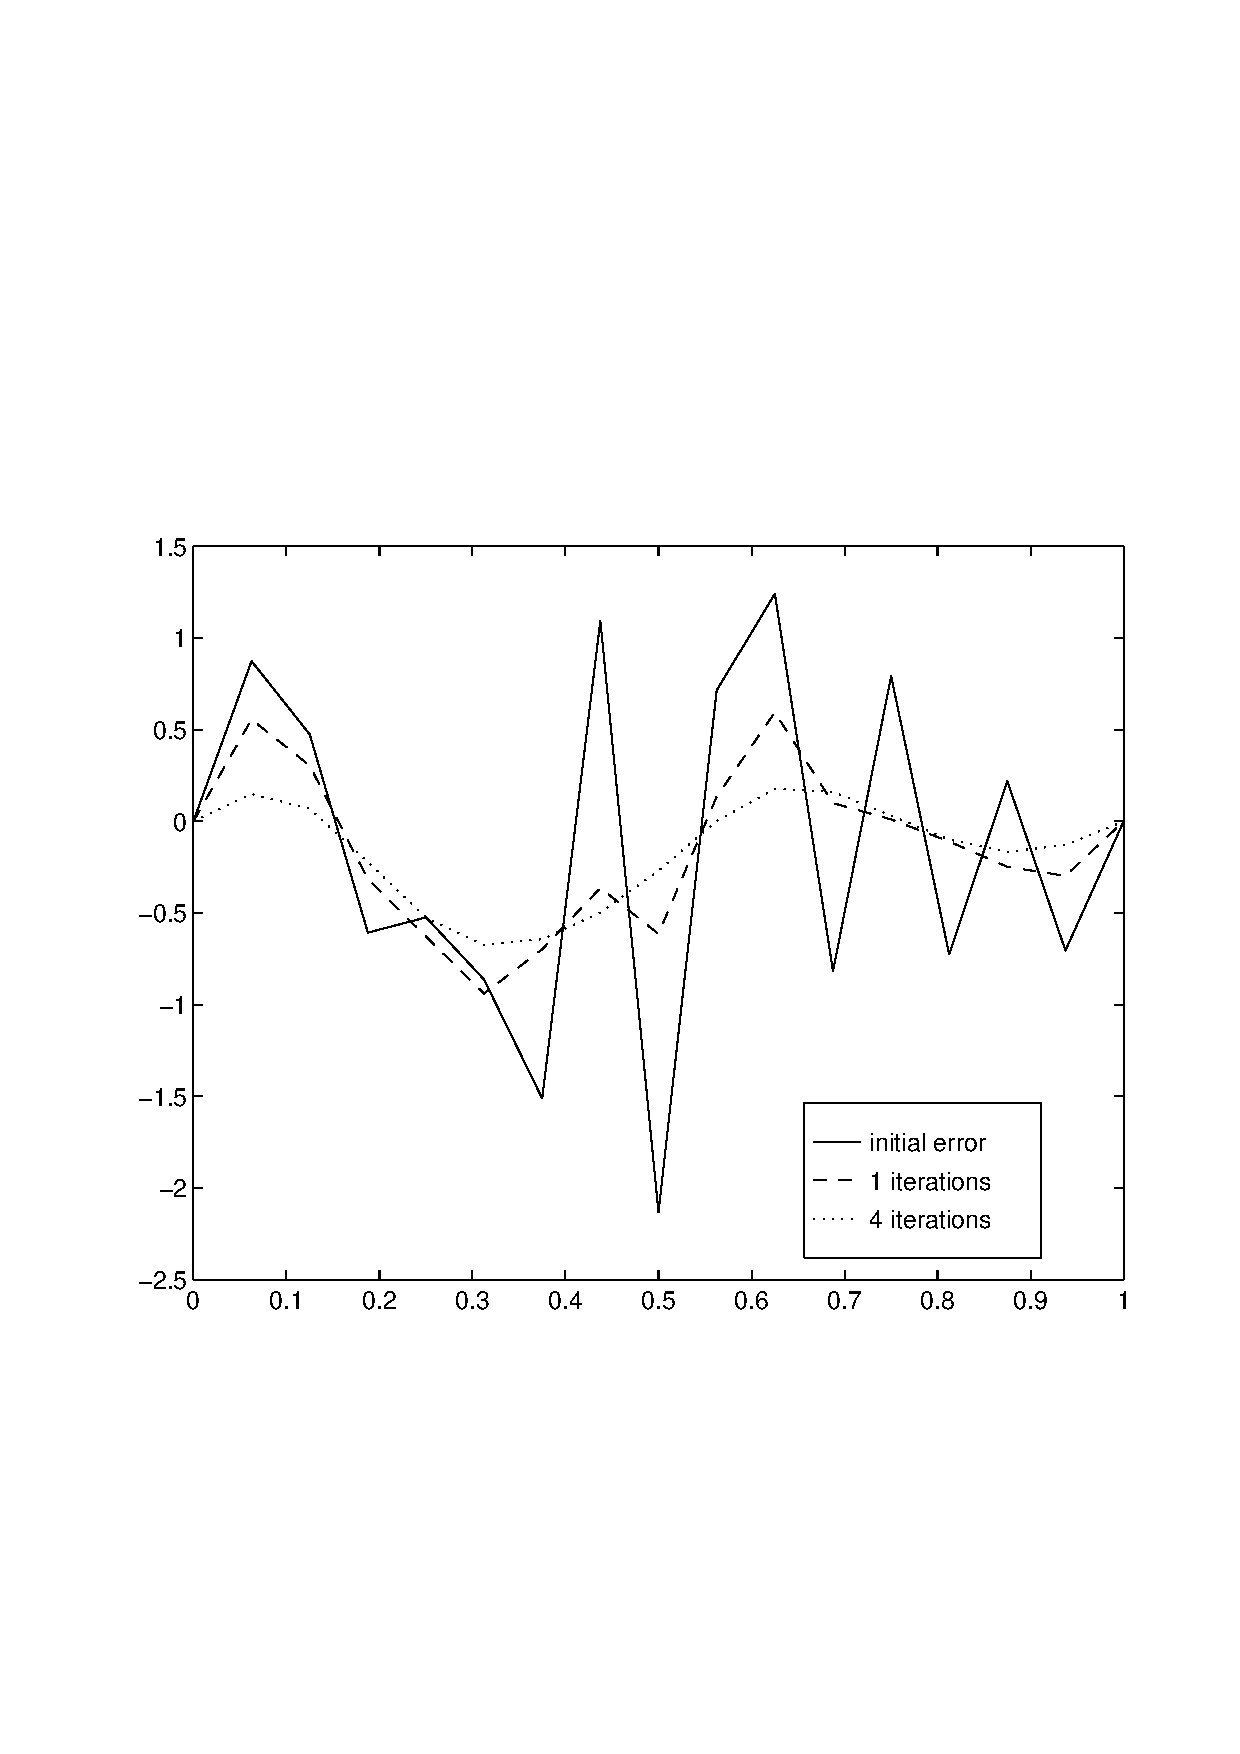
\includegraphics[height=5cm,width=3in]{pictures/smoothing.pdf}
\end{center}
\caption{The smoothing effect of the gradient descent method
\label{fig:smoothing}}
\end{figure}


In other words, the error function becomes a much smoother function
after a few such simple iterations.  This property of the iterative
scheme is naturally called {\it a smoothing property} and an iterative
scheme having this smoothing property is called a {\it smoother}.

The above two observations, especially the second one, concern the
most important property of the simple gradient descent method that we can
take advantage to get a much faster algorithm.


The gradient descent method can be written in terms of $S_{0}:\mathbb R^{N}\rightarrow \mathbb R^{N}$ satisfying
\begin{equation}
\label{jacobi1d}
\mu^{(1)}=(S_{0}b)={h\over 4} b,
\end{equation}
for equation \eqref{min} with initial guess zero.
If we apply this method twice, then
$$
\mu^{(2)}=S_1(b) = S_{0} b + S_0(b - A\ast(S_{0}b)),
$$
with element-wise form
\begin{equation} 
\begin{aligned}
\mu^{(2)}_{i} &={h\over 16}(b_{i-1}+6b_i+b_{i+1}).
\end{aligned}
\end{equation}
Then by the definition of convolution \eqref{con010}, we have
 \begin{equation}\label{eq:convS}
\mu^{(1)}= S_{0}\ast b \quad \mu^{(2)} = S_1 \ast b.
\end{equation}
with
\begin{equation}\label{eq:kernel-S1d}
S_{0} = {h\over 4},
\end{equation}
and 
\begin{equation}\label{eq:kernel-S2}
S_1={h\over 16}[1,6,1].
\end{equation} 

Hence we denote $S_0$ or $S_1$ as $S$.

Now for any given $\mu^{(0)}=\tilde{\mu}^{(0)}$, 
\begin{equation}
\begin{aligned}
&m=1,2,\cdots,2\nu\\
&\mu^{(m)}=\mu^{(m-1)}+S_0\ast(b-A\ast\mu^{(m-1)})
\end{aligned}
\end{equation}
$$\Leftrightarrow$$
\begin{equation}
\begin{aligned}
&m=1,2,\cdots,\nu\\
&\tilde{\mu}^{(m)}=\tilde{\mu}^{(m-1)}+S_1\ast(b-A\ast\tilde{\mu}^{(m-1)})
\end{aligned}
\end{equation}
we obtain $\mu^{(2\nu)}=\tilde{\mu}^{(\nu)}$ which means one step $S_1$ is equivalent to two steps of $S_0$.

\paragraph{Convergence and smoothing properties of GD}
Because of the extraordinary importance of this smoothing property, we
shall now try to give some simple theoretical analysis.  To do this,
we make use of the eigenvalues and eigenvectors of the matrix $A$.
\paragraph{Fourier analysis for the gradient descent method}
Our earlier numerical experiments indicate that the gradient descent
method has a smoothing property.  Based on our understanding of the
relation between the smoothness and the size of Fourier coefficients,
we can imagine that this smoothing property can be analyzed using the
discrete Fourier expansion.

Let $\mu$ be the exact solution of \eqref{min} and $\mu^{(m)}$ the result of
$m-th$ iteration from the gradient descent method \rf{1dRichardson}.  Then
$$
\mu-\mu^{(m)}=(1-\eta A\ast)(\mu-\mu^{(m-1)})=\ldots=(1-\eta A\ast)^m(\mu-\mu^{(0)}).
$$
Consider the Fourier expansion of the initial error:
$$
        \mu-\mu^{(0)}=\sum_{k=1}^N\alpha_k\xi^k.
$$
Then 
$$
        \mu-\mu^{(m)}=\sum_{k=1}^N\alpha_k(I-\eta A\ast)^m\xi^k.
$$
Note that $\eta=h/4$ and for any polynomial $p$
$$
p(A\ast)\xi^k=p(\lambda_k)\xi^k,
$$
we get
$$
        \mu-\mu^{(m)}=\sum_{k=1}^N\alpha_k(1-\eta\lambda_k)^m\xi^k
        =\sum_{k=1}^N\alpha_k^{(m)}\xi^k
$$
where 
$$
\alpha_k^{(m)}=\bigg(1-\sin^2{{k\pi}\over {2(N+1)}}\bigg)^m\alpha_k.
$$
For $k$ close to $N$, for example $k=N$,
note that 
$$
1-\sin^2{{N\pi}\over {2(N+1)}}=\cos^2{{N\pi}\over {2(N+1)}}
=\sin^2({\pi\over2}-{{N\pi}\over {2(N+1)}})
$$
implies
$$
|\alpha_N^{(m)}|=|\alpha_N|\sin^{2m}{{N+1-N}\over{N+1}}{\pi\over 2}
\le |\alpha_k|\bigg({{1}\over{N+1}}{\pi\over 2}\bigg)^{2m}
$$
which approaches to $0$ very rapidly when
$m\rightarrow\infty$. This means that high frequency components get
damped very quickly. 

However, for $k$ far away from $N$, for example $k=1$, note that
$$
\sin^2{{\pi}\over {2(N+1)}}\le \left({{\pi}\over {2(N+1)}}\right)^2
$$
implies
$$
|\alpha_1^{(m)}|= |\alpha_1| \bigg(1-\sin^2{{\pi}\over {2(N+1)}}\bigg)^m\ge  |\alpha_1|  \left(1-\left({{\pi}\over {2(N+1)}}\right)^2\right)^m
$$
which approaches to $0$ very slowly when
$m\rightarrow\infty$. 

This simple analysis clearly justifies the smoothing property that has
been observed by numerical experiments.

%\newpage

\begin{figure}[!ht]
\setlength{\abovecaptionskip}{0pt}
\setlength{\belowcaptionskip}{0pt}
\includegraphics[width=5cm]{figures/jianhongu0.png}\qquad
\includegraphics[width=5cm]{figures/jianhongu1.png}\qquad
\includegraphics[width=5cm]{figures/jianhongu2.png}\qquad
\includegraphics[width=5cm]{figures/jianhongu3.png}\qquad
\includegraphics[width=5cm]{figures/jianhongu4.png}\qquad
\includegraphics[width=5cm]{figures/jianhongGDerror.png}
\caption{\footnotesize{ $u-u^0$, $u-u^1$, $u-u^2$, $u-u^3$, $u-u^4$}}
\label{fig:Hmesh}
\end{figure}

%\begin{figure}[!ht] 
%\centering
%\includegraphics[width=5cm,height=4cm]{figures/jianhongu0.png}
%\caption{ $u^0$}
%\label{fig:u0j}
%\end{figure}
%\begin{figure}[!ht] 
%\centering
%\includegraphics[width=5cm,height=4cm]{figures/jianhongu1.png}
%\caption{ $u^1$}
%\label{fig:u1j}
%\end{figure}
%\begin{figure}[!ht] 
%\centering
%\includegraphics[width=10cm,height=8cm]{figures/jianhongu2.png}
%\caption{ $u^2$}
%\label{fig:u2j}
%\end{figure}
%\begin{figure}[!ht] 
%\centering
%\includegraphics[width=10cm,height=8cm]{figures/jianhongu3.png}
%\caption{ $u^3$}
%\label{fig:u3j}
%\end{figure}
%\begin{figure}[!ht] 
%\centering
%\includegraphics[width=10cm,height=8cm]{figures/jianhongu4.png}
%\caption{ $u^4$}
%\label{fig:u4j}
%\end{figure} 

\paragraph{An intuitive discussion} 
The gradient descent method is oftentimes called {\it local relaxation}
methods. This name refers to the fact that what that
algorithm does is just trying to correct the residual vector locally
at one nodal point at a time (recall that $\mu_j\approx u(x_j)$).
This local relaxation procedure is then effective to the error
components that are local in nature.  Incidentally, the nonsmooth or
high frequency component which oscillates across one or few grid
points have a strong local feature.  Therefore, it is not surprising the
 gradient descent  iteration can damp out these
nonsmooth components more easily.  This method is very inefficient
for relatively smoother components in the error since a smoother
function is more globally related in nature.

